%%%%%%%%%%%%%%%%%%%%%%%%%%%%%%%%%%%%%%%%%%%%%%%%%%%%%%%%%%%%%%%%%%%%%%%%%%%%%% %%
%12345678901234567890123456789012345678901234567890123456789012345678901234567 89
%        1         2         3         4         5         6         7 8

\documentclass[letterpaper,10pt,conference]{ieeeconf}  % Comment this line out if you needa4paper
\usepackage{amsmath}
\usepackage{amssymb}
\usepackage{comment}
\usepackage{todonotes}
%\documentclass[a4paper,10pt,conference]{ieeeconf}        % Use this line for a4 paper

\IEEEoverridecommandlockouts                              % This command is only needed if
                                                          % you want to use the \thanks command

\overrideIEEEmargins                                      % Needed to meet printer requirements.

% See the \addtolength command later in the file to balance the column lengths
% on the last page of the document

% The following packages can be found on http:\\www.ctan.org
\usepackage{graphics} % for pdf, bitmapped graphics files
\usepackage{epsfig} % for postscript graphics files
%\usepackage{mathptmx} % assumes new font selection scheme installed
%\usepackage{times} % assumes new font selection scheme installed
\usepackage{amsmath} % assumes amsmath package installed
%\usepackage{amssymb}  % assumes amsmath package installed

\title{\LARGE \bf
 Learning and inference with a compositional hierarchical representation of 3D object shape
}


\author{Dominik Belter, Marek Kopicki, Ales Leonardis and Jeremy L. Wyatt% <-this stops a space
% \thanks{}% <-this % stops a space
% \thanks{D. Belter, M. Nowicki and P. Skrzypczy\'nski are with the Institute of Control and 
%  Information Engineering, Poznan University of Technology, ul. Piotrowo 3A 60-965 Pozna\'n, Poland,
%  {\tt\small \{name.surname\}@put.poznan.pl}}%
}


\begin{document}


\maketitle
\thispagestyle{empty}
\pagestyle{empty}


%%%%%%%%%%%%%%%%%%%%%%%%%%%%%%%%%%%%%%%%%%%%%%%%%%%%%%%%%%%%%%%%%%%%%%%%%%%%%% %%
\begin{abstract}
Modelling of object shape is an essential pre-cursor to any method for object manipulation. In this paper we present a method for learning compositional hierarchical representations of 2.5D and 3D object shape. These are representations that consist of a hierarchy of parts. We present novel algorithms for learning and inference. We empirically demonstrate the ability to learn these representations from real depth data, and to fill in missing information caused by self-occlusions. We also demonstrate the ability of the hierarchy to model variable shape, and to share parts across different objects and object categories.
\end{abstract}


%%%%%%%%%%%%%%%%%%%%%%%%%%%%%%%%%%%%%%%%%%%%%%%%%%%%%%%%%%%%%%%%%%%%%%%%%%%%%% %%

\section{Introduction}

Grasping and manipulation actions that are generalisable across objects require representations of object shape that are expressive of and robust to variations in shape. These representations must have several properties.  Features, for example, must be shared across objects and object categories, as well as being robust to variability. In addition, global object shape must be inferrable from partial views, and missing parts must be inferred reliably. Compositional hierarchies are a particular class of representations that have proven themselves with respect to these properties in the domain of object categorisation from intensity images. In these representations an object or image is represented as a hierarchy of parts learned in a statistical manner. In this paper we develop a learning and inference framework for compositional hierarchical models of 3D shape. This takes view based depth images as input, rather than either intensity images, or complete shape data. We show empirically that it has properties of shareability, robustness to variability, and the ability to approximately infer missing shape information. We offer the framework as a promising representation to support future work in generalisable grasping and manipulation.

Our approach to objects represantation is based on the models which explain visual processing in human cortex~\cite{Riesenhuber1999}. According to these models the visual processing is hierarchical and all layers are learned. First layers of the hierarchy are position and scale invariant. The higher layers of the hierarchy build invariance to the viewpoint~\cite{Spehr2015}. Also the receptive fields increase with the layer of the hierarchy. The HMAX model~\cite{Serre2007} assumes that the inference process is feedforward to obtain fast objects recognition.

Our approach differs to biological counterparts. We build view invariance of parts from the very beginning. Our choice is motivated by the application. Our goal is to learn representation of objects from minimal number of examples. For view-variant representations the objects used for training should be observed from many viewpoints to build sufficient vocabulary. The number of parts which are required to represent the object is acceptable for 2D models~\cite{Fiedler2014}. Unfortunatelly, it explodes if the vocabulary of 3D parts is built. In our approach we have to run optimization which aligns parts in 3D whenever similarity between parts has to be computed but we show that this can be performed efficiently using Umeyama method. The additional advantage of our approach is the small number of parts in vocabulary which does not require GPU implementation.

\section{Related work}

\section{Learning}

\begin{figure}[t]
 \centering
\includegraphics[width=1.0\columnwidth]{../images/hierarchyParts.eps}
\caption{An illustration of a portion of our learned hierarchical representation of 3D objects. Within the $i$-th layer vocabulary $\Omega^i$ each word represents a 3D shape. Arrows represent compositional relations between parts.}
 \label{hierarchyParts}
\end{figure}

Our overall procedure for learning a compositional shape hierarchy is as follows. In this paper we build two linked hierarchies, one where parts are learned from single views, and one where parts are learned from many views. The view independent layers are built on top of the second view dependent layer. The hierarchy is learned layer by layer, with each layer consisting of a part vocabulary. Each part in a vocabulary is also called a word. Instantiations of parts caused by data are called realisations. 

\begin{figure}[t]
 \centering
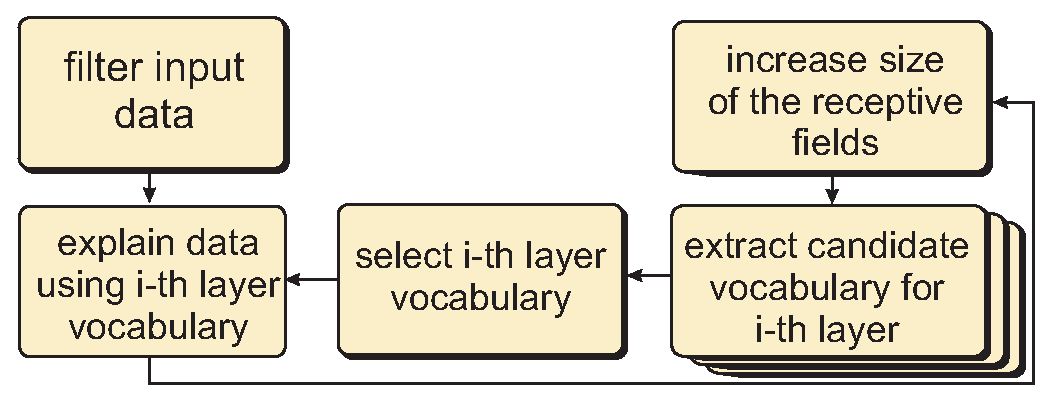
\includegraphics[width=0.9\columnwidth]{../images/learningGeneral.eps}
\caption{General procedure of learning the hierarchical representation of objects}
 \label{hopProc}
\end{figure}

First, starting with a layer consisting of a single seed part, we learn two additional layers of parts from depth images obtained from particular viewpoints. The receptive fields for these parts are areas of the image plane. Then, to learn the three view-independent layers above these, the hierarchy brings together different views of the same parts so as to create view independent 3D shape parts. The receptive fields for these parts are 3D volumes. It should be noted that the first three layers are view dependent in that they are each learned from data from a single viewpoint. For maximum generalisation, however, the part representations themselves are view-invariant, achieved by attaching a frame of reference to the part itself, rather than to the camera frame.  The subsequent view-invariant layers are created from multiple depth images. We thus switch from receptive fields defined as intervals on the image plane for the view dependent layers, to volumetric receptive fields defined as intervals on the 3D workspace. At each layer, each dimension of the receptive field for a part trebles. This means that parts in a layer $i$ are compositions of 9 or 27 parts from layer $i-1$.  Each layers is learned from the layer below. The procedure is repeated until the desired number of layers is obtained. In general the receptive field of the last layer should cover the whole object. A visualisation of a portion of a learned hierarchy is shown in Figure XX.  

\subsection{Learning the view-variant layers}

The general procedure for learning is presented in Fig.~\ref{hopProc}. To pre-process the images we perform background subtraction and denoising with a $7 \times 7$ median filter.  Then we compute the normal vector for each point in the image. To compute this normal vector we use Principal Component Analysis (PCA). We compute normal vectors using a 7$\times$7 window. Because PCA does not work properly on edges we detect two surfaces inside the sliding window. Then, we remove all points which don't belong to the dominant surface inside the sliding window.

Layer 1 is simply a single atomic planar patch. To extract planar patches from a given depth image, we divide the image into a regular grid. Each cell (5$\times$5 pixel patch) corresponds to a receptive field for the first layer. The surface of the object as divided into receptive fields is presented in Fig.~\ref{recFields1}. Given the normals for the points we now find the best orientation of the planar patch for each receptive field.  This estimation process creates a piecewise planar interpretation of the image. During learning, this is performed on every image in the training set, so as to create a large set of realisations.

\begin{figure}[t]
 \centering
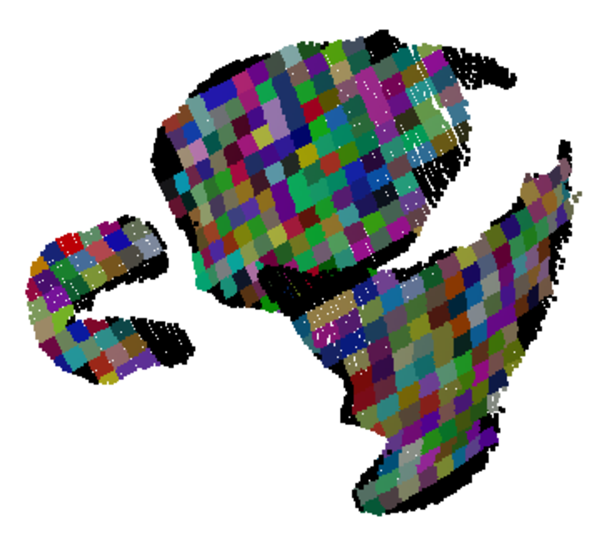
\includegraphics[width=0.5\columnwidth]{../images/recFields1.eps}
\caption{A point cloud obtained from single camera view divided into first layer receptive fields. Each colour represents a receptive field. Black points are not used to compute planar patches}
 \label{recFields1}
\end{figure}

To create layer 2, these planar part realisations are first grouped into receptive fields consisting of 9 planar patches (Fig.~\ref{word}).\footnote{If any receptive field does lie entirely within the surface of the object the sub-part is represented by the background. The minimal number of non-background sub-parts in the second layer word (part) is set to four. This is the minimal number of points required to compute similarity between parts.} These are the candidate parts for the $2^{nd}$ layer, of which a subset are selected to form the actual parts of layer 2. This compression underpins the generalization properties of the hierarchy, and is achieved by clustering. To represent each cluster the part at the centre of the cluster is chosen.

\begin{figure}[t]
 \centering
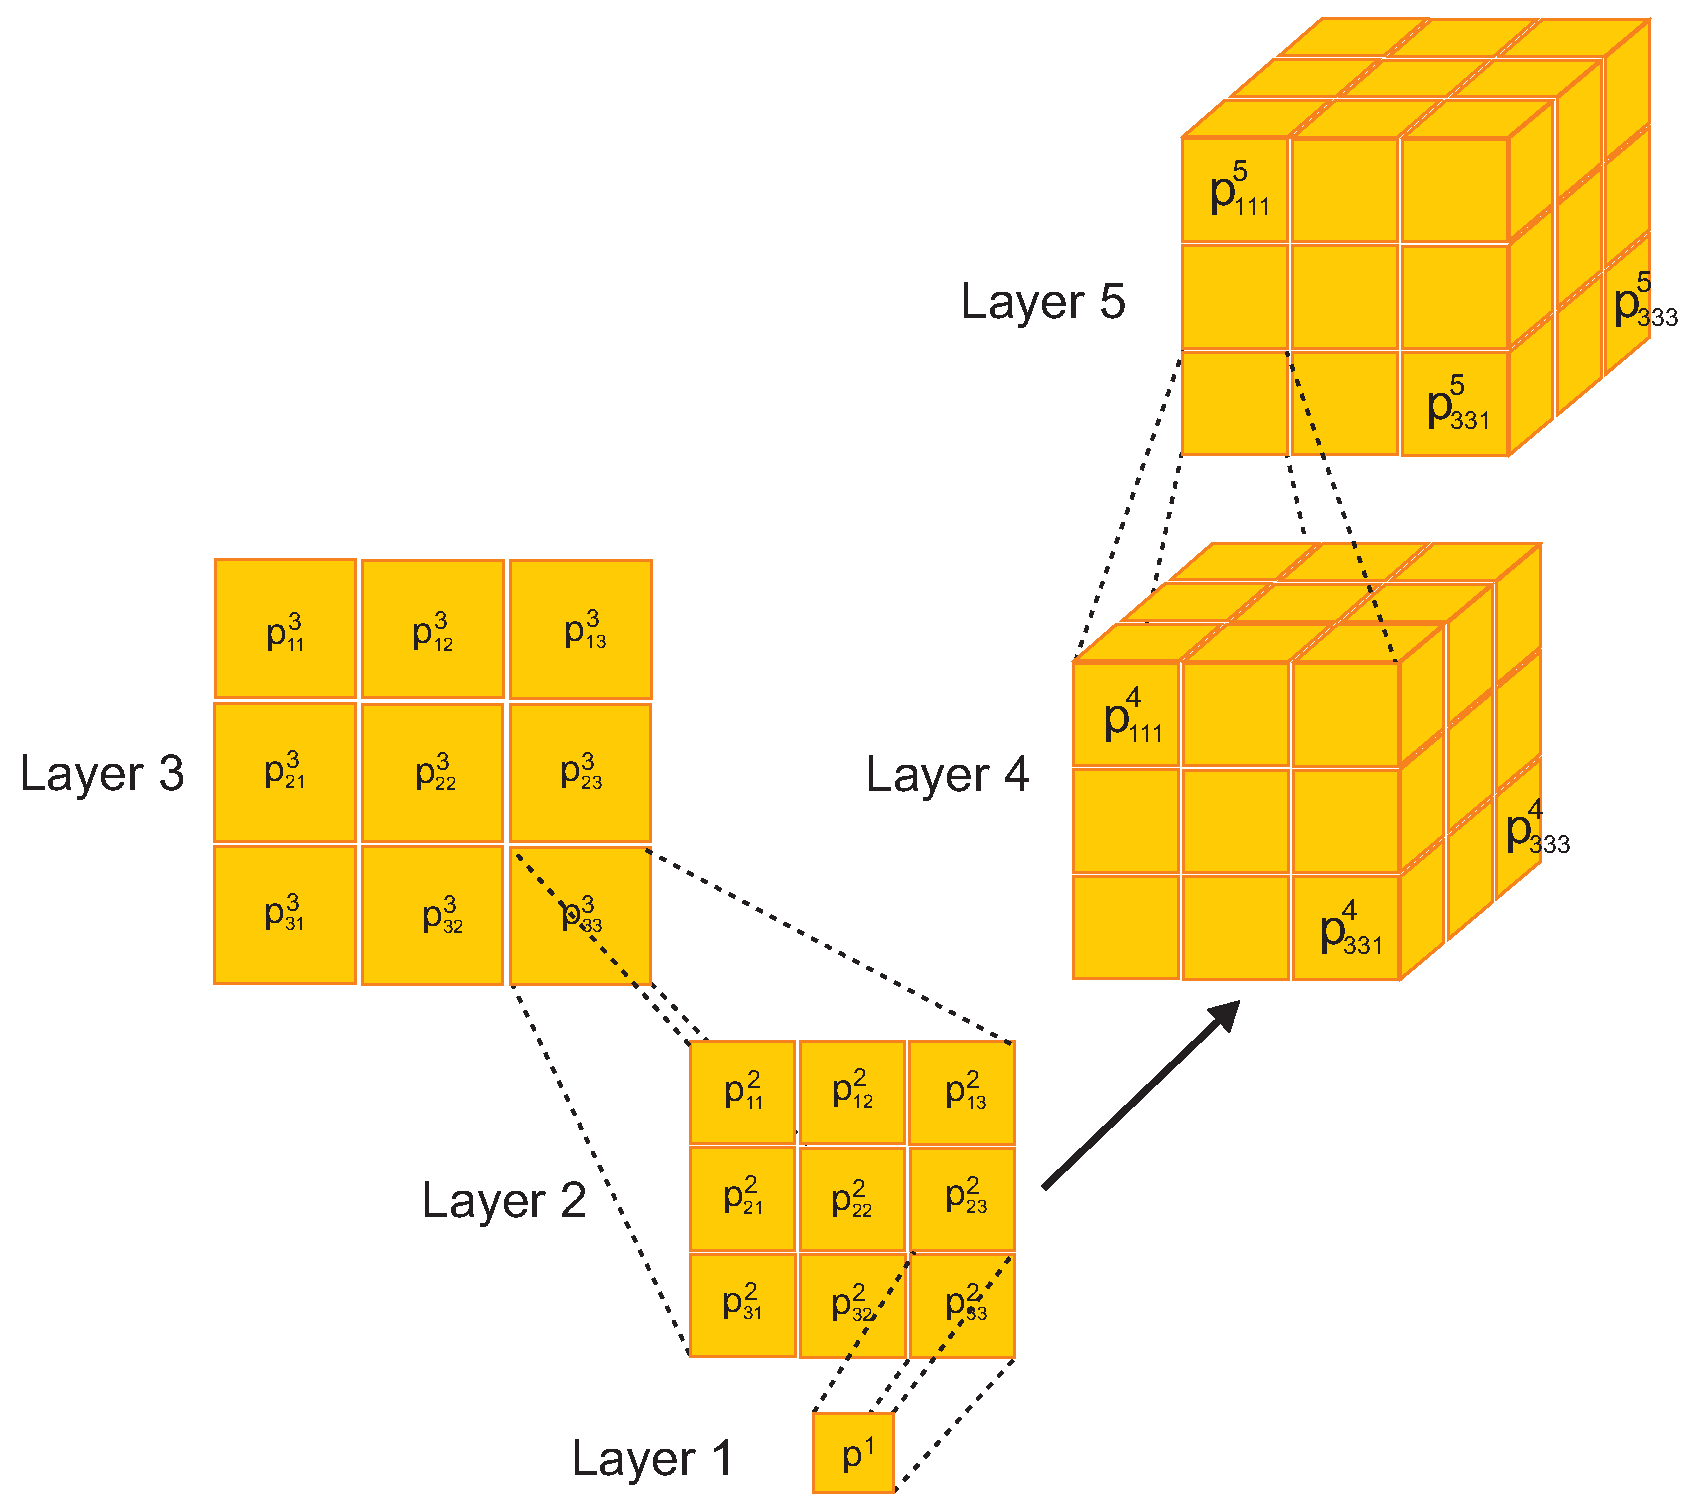
\includegraphics[width=0.9\columnwidth]{../images/hierarchy.eps}
\caption{Representation of receptive fields in the hierarchy. Each receptive field at the lowest layer is $5 \times 5$ pixels. Arrows represent the surface normals for those planar patches. First three layers of the hierarchy are defined on the image plane. The next two layers are volumetric.}
 \label{word}
\end{figure}

The parts in the second layer are then again fitted to from all images used for training the hierarchy. The variability of the parts used for learning is increased by introduction overlapping receptive fields. Overlapping receptive fields also allow us to deal with problems arising from the  partition of the image into a regular grid. Because of this partition the camera pose relative to the object strongly influences the position of the receptive fields on the object's surface. This causes data loss on the edges of the object. If the receptive field is shifted the part computed for the surface may cover only the object, the background or both. The position of the receptive field influences the part detected on the image. By using overlapping receptive field the number of hypothesis about each point on the image plane increases. These overlapping receptive fields are presented in Fig.~\ref{overlap}. The stride at layer $i$ is simply the width of a part at layer $i-1$. This means that each pixel might be explained by three different parts. 

This procedure---of fitting parts, enumerating realisations, and clustering---is repeated. At each stage the  vocabulary for the $i^{th}$ layer is used to find all the realisations in the depth data for all images. Then candidate parts for the $i+1^{th}$ layer are formed from receptive fields that group these realisations. Finally, we select the $i+1^{th}$ layer vocabulary by clusterization of parts (words) in the vocabulary. 

\begin{figure}[t]
 \centering
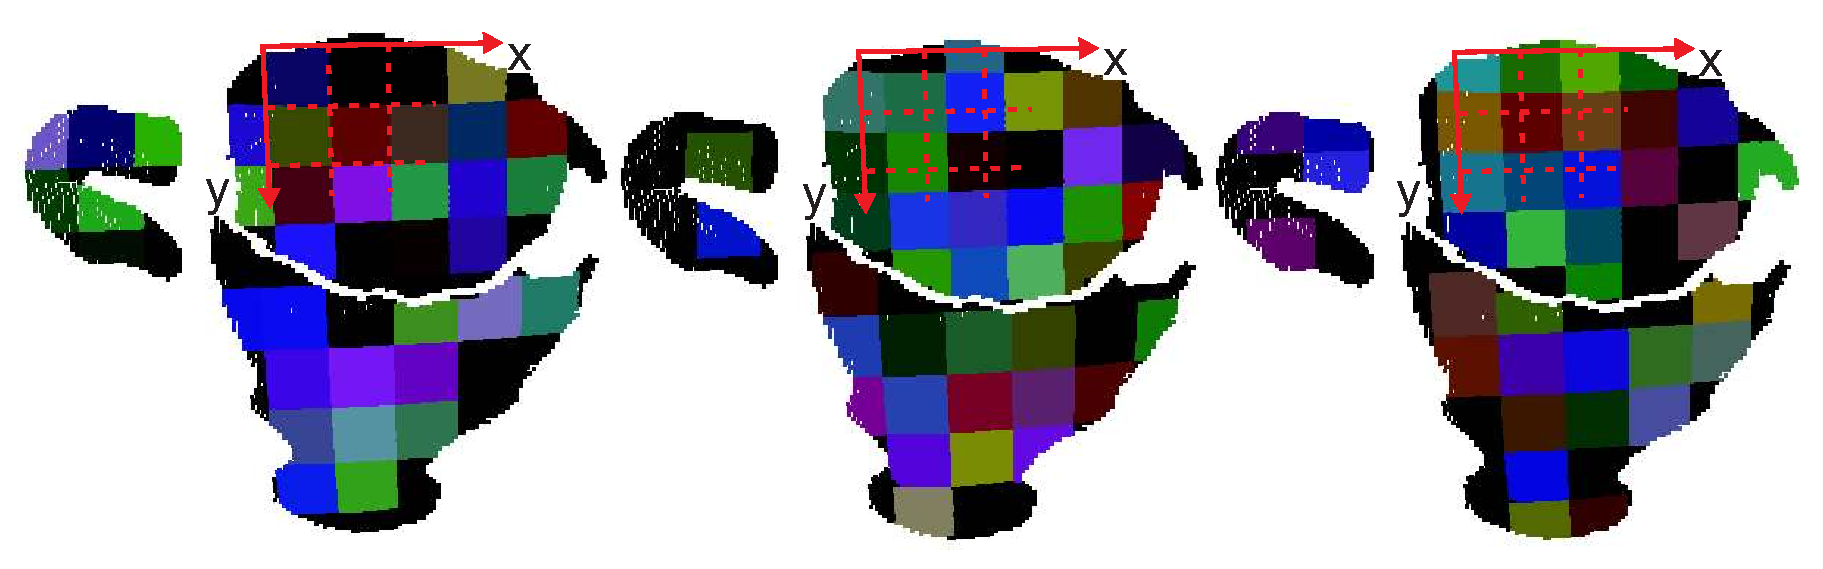
\includegraphics[width=0.99\columnwidth]{../images/overlap.eps}
\put(-222,62){a} \put(-142,62){b} \put(-60,62){c}
\caption{Overlapping receptive fields: the receptive field shifts by 0\% (a), 33\% (b) and 66\% (c)}
 \label{overlap}
\end{figure}

For this purpose Hierarchical Agglomerative Clustering is used~\cite{Manning2008}. We merge clusters according to the similarity between parts. We stop the procedure if the distance (similarity) between parts $d^c$ is bigger than a threshold. Moreover, after each step which merges two clusters we compute maximal distance $d^c_{\rm max}$ between parts inside each cluster. If the distance inside the cluster is bigger than threshold the cluster is split in two, thus limiting the maximum intra-cluster distance. The number of obtained parts in the vocabulary depends on two parameters: $d^c$ and $d_{\rm max}$. Similarity between two view dependent parts $p_A$ and $p_B$ is defined by the distance metric $d_{\rm VD}$:

\begin{equation}
\label{distVD}
 d_{\rm VD}=\sum_{i,j}^N ( c_1 d(p_A^{\rm ij}, p_B^{\rm ij}) + c_2 acos({\bf N}_A^{\rm ij} \cdot {\bf N}_B^{\rm ij})),
\end{equation}

where $d(p_A^{\rm ij}, p_B^{\rm ij})$ is the Euclidean distance between the centres of corresponding patches, $N_A^{\rm ij}$ and $N_A^{\rm ij}$ are the corresponding normal vectors in parts A and B, and $c_1$ and $c_2$ are constant values which scale the Euclidean distance against the angles between normal vectors. The distance $d_{\rm VD}$ is computed taking into account corresponding sub-parts. If both sub-parts are background the distance value is not increased. If one of the corresponding sub-part is background and the second corresponds to planar patch the distance $d_{\rm VD}$ is increased by constant value $c_3$.

As stated, the parts are created from view specific data, but the frame of reference for each part is attached to the part. This means that that we can distinguish between planar, concave, convex, and other local shapes, independent of the angle of observation. This in turn significantly reduces the number of parts in the hierarchy. In contrast to an equivalent hierarchy for 2D intensity images~\cite{Fiedler2014}, the discretization of normal vectors is not required in hierarchy of 3D parts. We store continuous values of the normal vector. This permits learning of the hierarchy from small numbers of exemplars. To obtain this frame of reference for each part we solve the following optimization problem:

\begin{equation}
\label{optVI}
 \arg\min_{\bf T} d_{\rm VD}({\bf T}),
\end{equation}

where ${\bf T}$ is an SE(3) rigid body transformation, $d_{\rm VD}({\bf T})$ is the distance metric (\ref{distVD}) computed for part $p_A$ and part $p_B$ transformed by ${\bf T}$. To find the rigid body transformation ${\bf T}$ which aligns part A and part B we use the Umeyama method~\cite{Umeyama1991}. The Umeyama method finds the optimal transformation ${\bf T}$ (root mean squared error is minimized) between points with known correspondence. To find correspondences between patches in parts we perform exhaustive search. We take into account 8 possible rotations of parts around central element. Note that we don't rotate the part in 3D space. We modify correspondences between elements only. After this step the parts are aligned by the Umeyama method and the similarity distance $d_{\rm VD}({\bf T})$ between parts is computed. 

\begin{figure}[t]
 \centering
 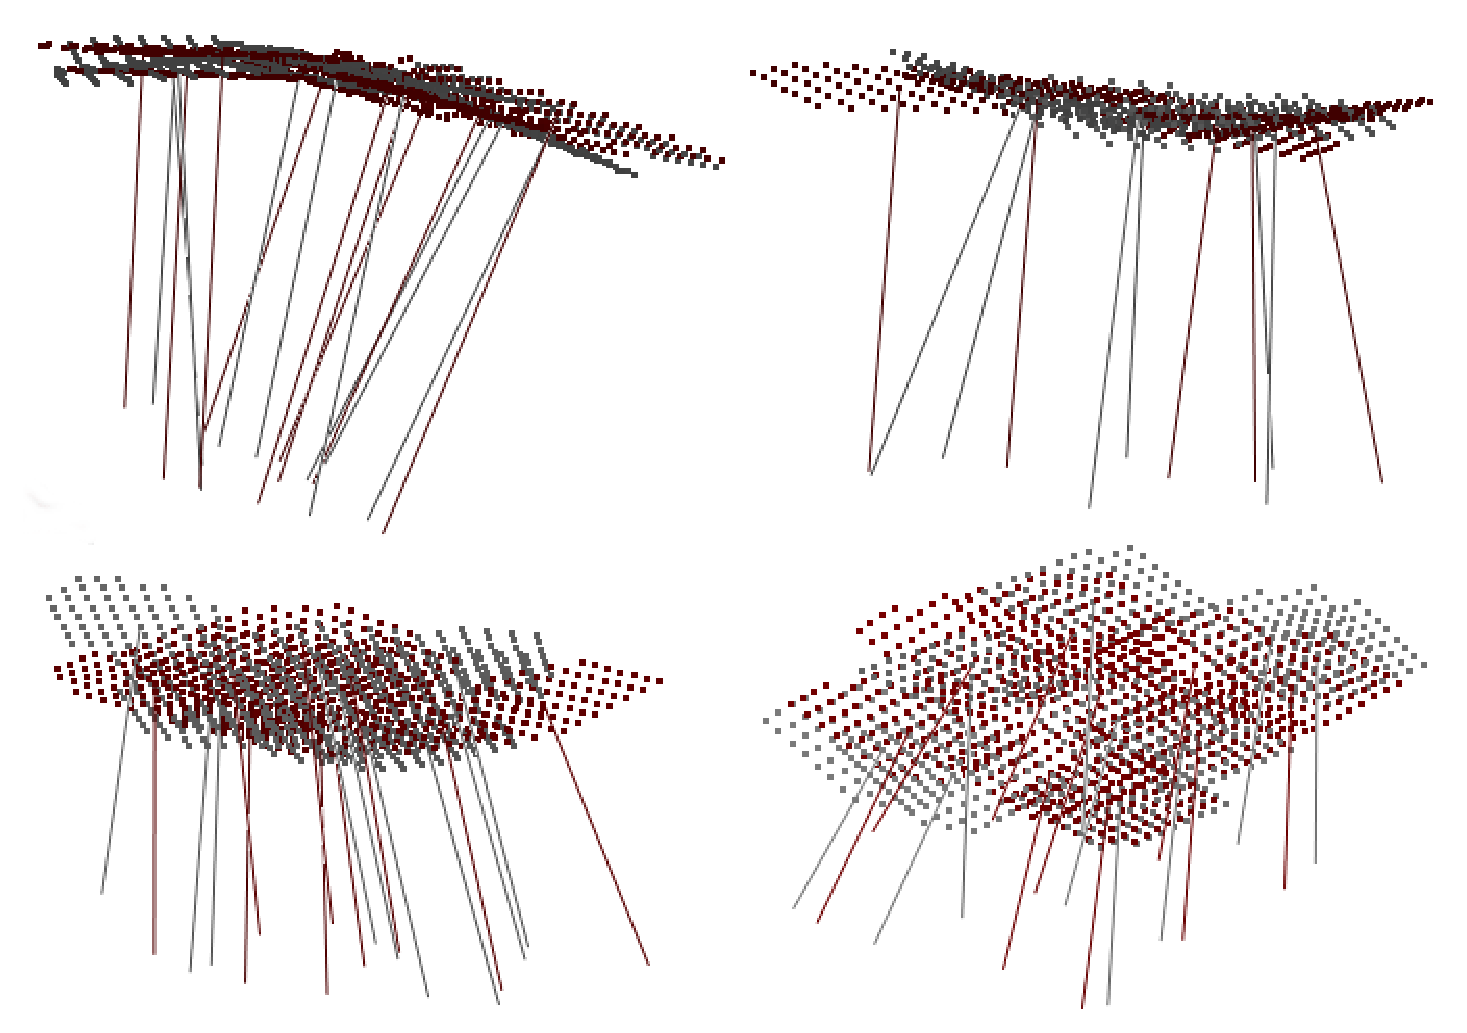
\includegraphics[width=0.95\columnwidth]{../images/parts2ndLayer.eps}
 \caption{Alignment of parts from the second layer. Gray -- part A ($p_A$), red -- part B ($p_B$)}
 \label{parts2ndLayer}
\end{figure}

To align parts from the the $i+1^{th}$ layer the hierarchical structure of parts has to be used. Parts in higher layers are created using parts from lower layers. Thus, the parts of the first layer are represented by a single point, parts of the second layer are represented by 9 points, third layer parts by 81 points, and in general the size $s_{\rm i+1}$ of the $i+1$ layer part is $9s_i$. To obtain the point cloud and to find correspondences and compute the optimal alignment the subparts have to be recursively represented by points with normal vectors.

An example alignment for parts from the second layer is presented in Fig.~\ref{parts2ndLayer}. We represent each planar patch as a point cloud. The data points for each part do not match perfectly. Small differences in the positions and orientations of sub-parts and even missing sub-parts occur, but can be dealt with by the alignment procedure. This property is what enables the hierarchy to generalize learned models and classify parts properly despite sensor noise.

\begin{figure}[t]
 \centering
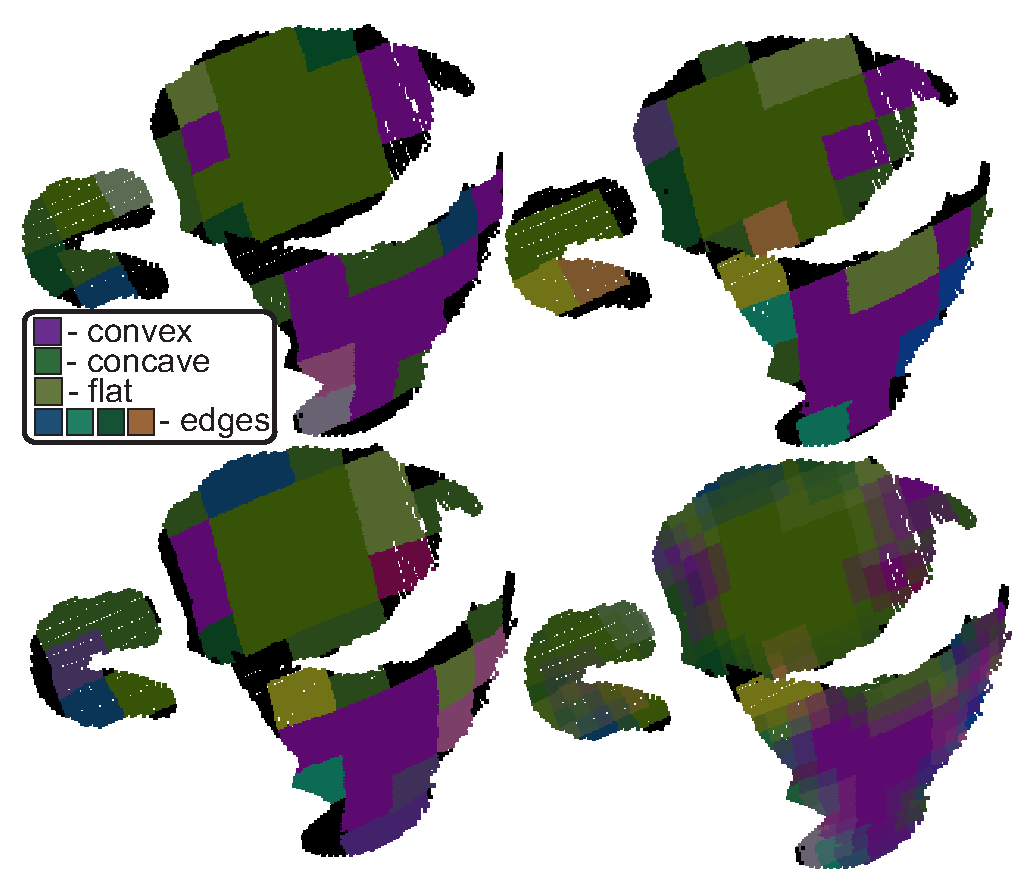
\includegraphics[width=0.95\columnwidth]{../images/2ndLayer.eps}
\put(-215,182){a} \put(-102,182){b}
\put(-215,82){c} \put(-102,82){d}
\caption{Clusterization results for the second layer. Parts from the same group have the same colour on the object visualization: overlap 0\% (a), overlap 33\% (b), overlap 66\% (a), combination of hypotheses (d)}
 \label{2ndLayer}
\end{figure}

The variability of sub-parts is encoded in the clusters. These clusters are created without supervision, and the algorithm generates natural groups of planar, concave and convex parts. Other groups contain various elements which represent edges in the depth image. These parts contain sub-parts created from planar patches and background elements. The example clusterization results--- given overlapping receptive fields and a single view-point---are presented in Fig.~\ref{2ndLayer}. The hierarchy distinguishes between various parts, but groups them if the local shape is similar. Some surfaces are misclassified. The size of the receptive field in the second layers is small and the noise of the sensor plays an important role here. However, multiple hypotheses about the parts help to deal with this problem (Fig.~\ref{2ndLayer}).

\subsection{Data explanation using $i$-th layer vocabulary}

\begin{figure}[t]
 \centering
\includegraphics[width=0.95\columnwidth]{../images/explanation2ndLayer.eps}
\put(-232,172){a} \put(-232,77){b}
\caption{Explanation of data using the vocabulary from the second layer without compression (659 parts) (a) and with compression (38 parts) (b)}
 \label{explanation2ndLayer}
\end{figure}

In the next step the input data is explained using the obtained $i$-th layer vocabulary. We explain the image using representative parts only. Thus, some areas of the image are replaced by $i$-th layer representative parts. This enables compression of the input data as well as generalization. Using information about camera pose, the parts can be moved into 3D space and reconstruct the object. Then, we can visually check the compression and clusterization results. The representation of the object created from the second layer vocabulary is presented in Fig.~\ref{explanation2ndLayer}. In Fig.~\ref{explanation2ndLayer}a a representation of the object created from 659 parts is presented. In this case the compression rate is set to 0\%. In Fig.~\ref{explanation2ndLayer}b the representation of the object is created from just 38 parts. The compression rate for this layer is 5.8\%. Despite the big reduction in the number of parts the explanation of the input data is still precise. Moreover, the normals vary more smoothly for the object created from the compressed vocabulary. This property arises from the clusterization. The variation of the shapes inside clusters which is also caused by the sensor noise is represented by the ``average'' part in the centre of the cluster.

\begin{figure}[t]
 \centering
 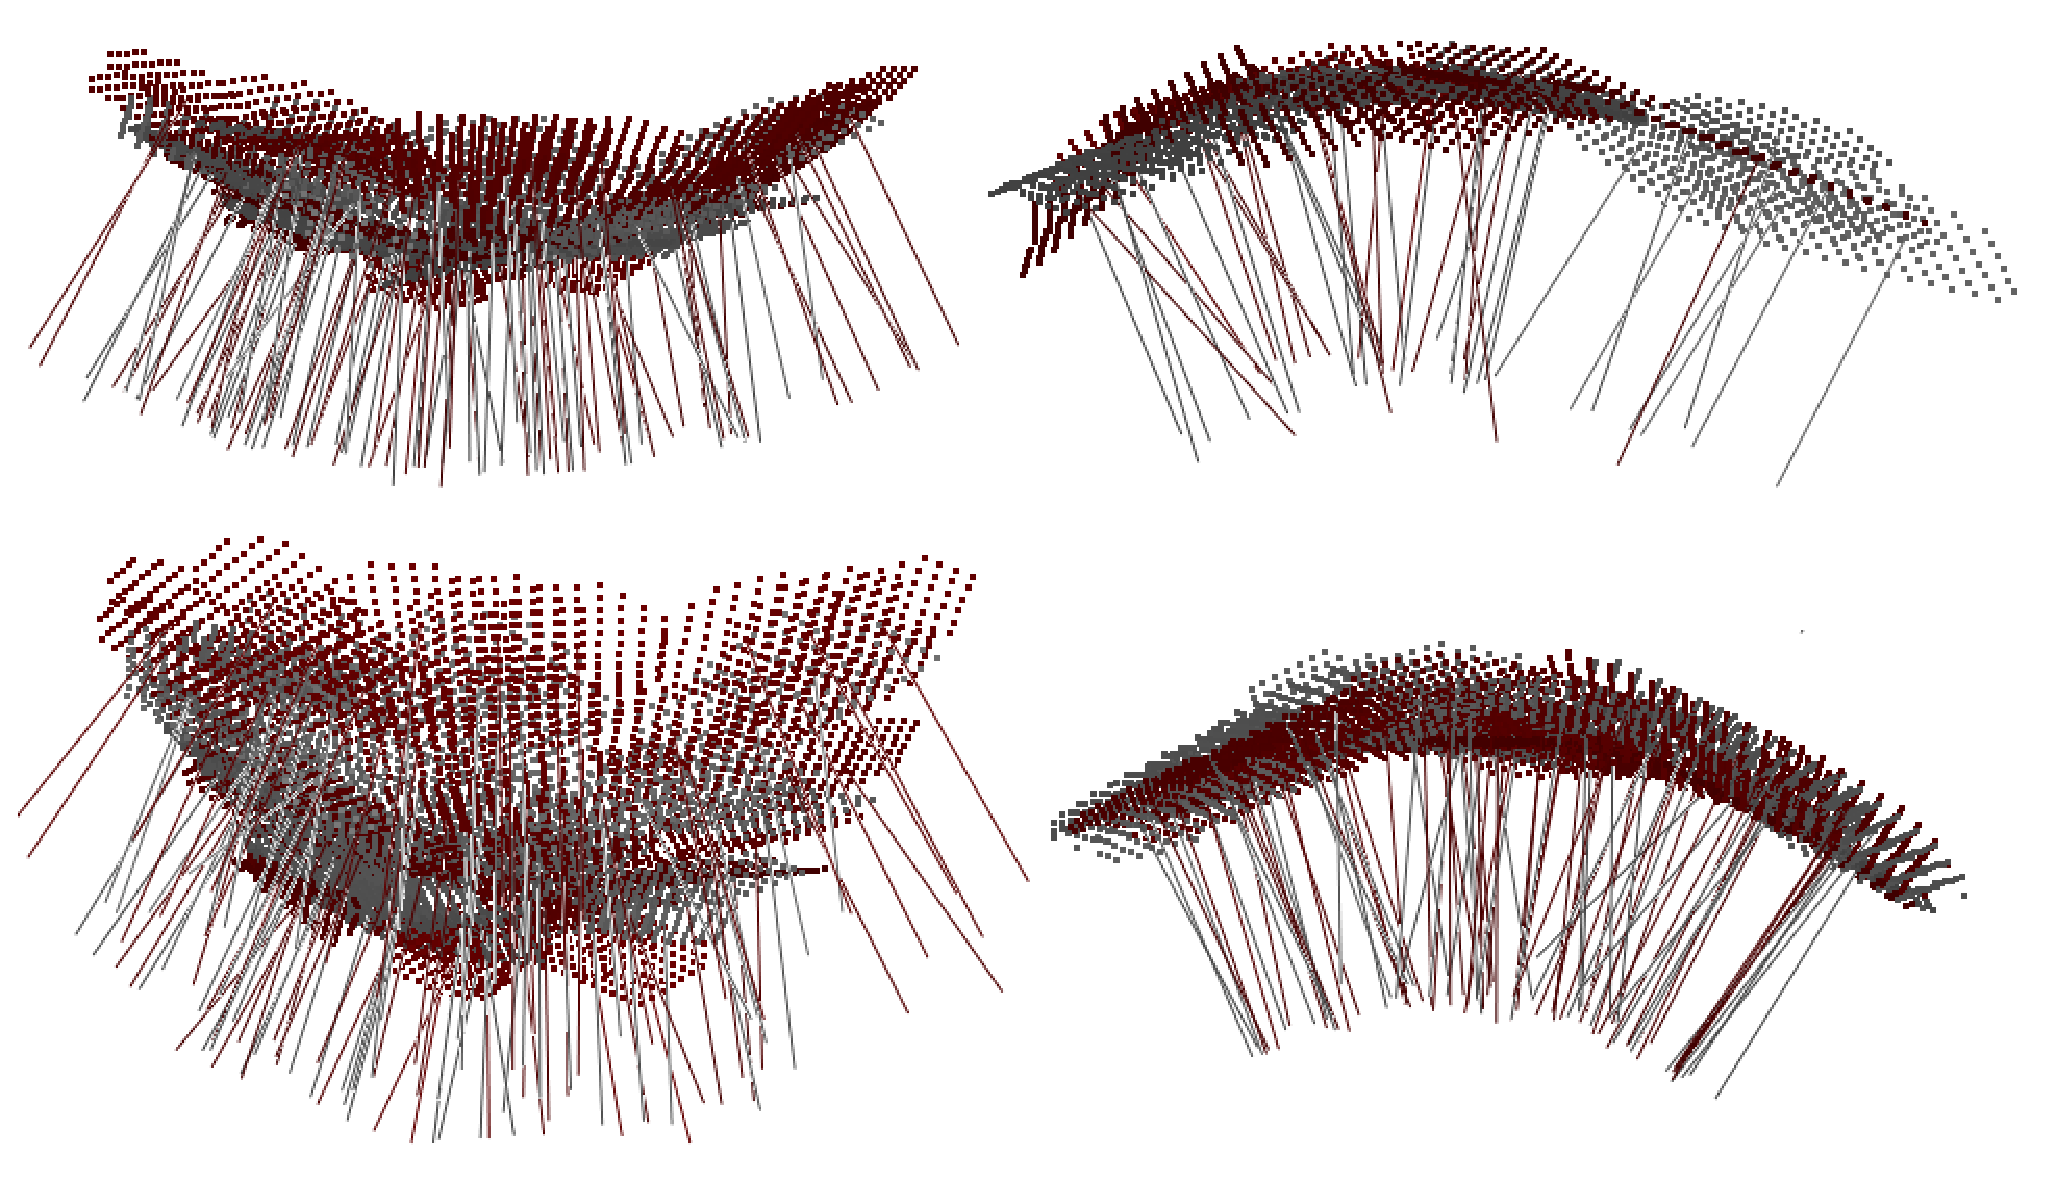
\includegraphics[width=0.95\columnwidth]{../images/parts3rdLayer.eps}
 \caption{Alignment of parts from the third layer. Gray -- part A ($p_A$), red -- part B ($p_B$)}
 \label{parts3rdLayer}
\end{figure}

\begin{figure}[t]
 \centering
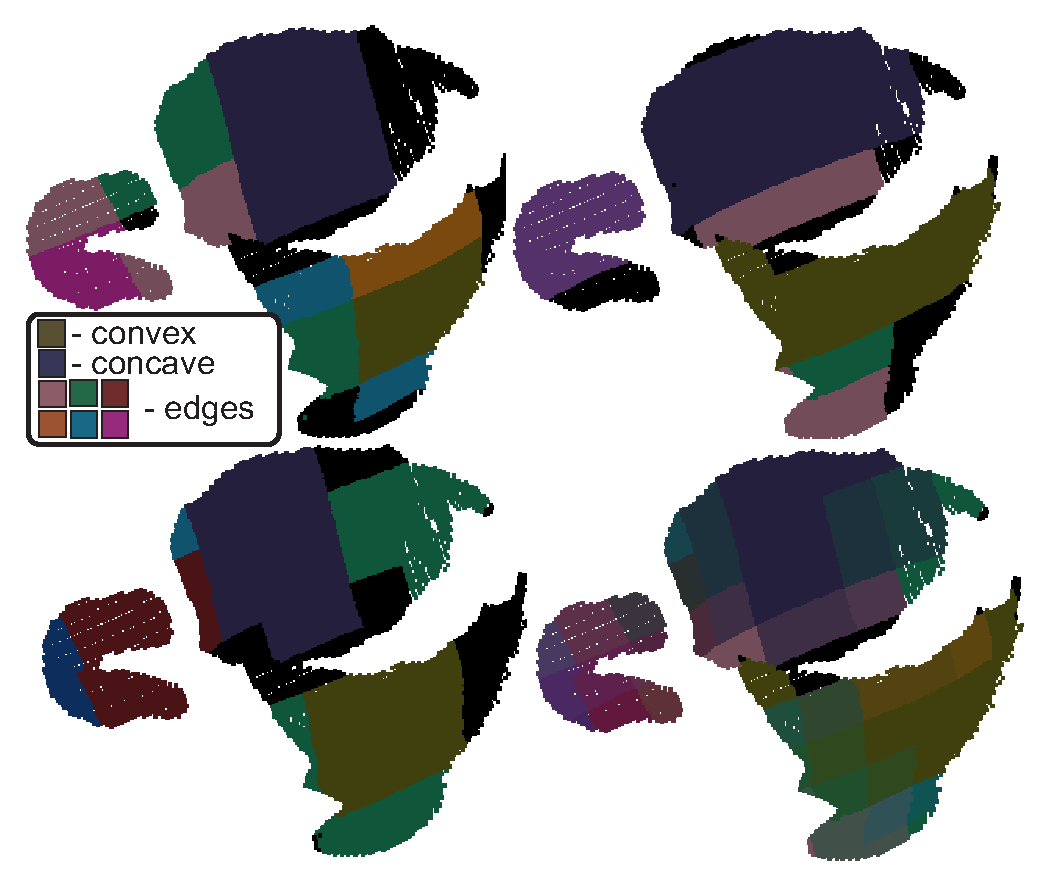
\includegraphics[width=0.95\columnwidth]{../images/3rdLayer.eps}
\put(-215,182){a} \put(-102,182){b}
\put(-215,82){c} \put(-102,82){d}
\caption{Clusterization results for the second layer. Parts from the same group have the same colour in the object visualization: overlap 0\% (a), overlap 33\% (b), overlap 66\% (a), combination of hypotheses (d)}
 \label{3rdLayer}
\end{figure}

\begin{figure}[t]
 \centering
\includegraphics[width=0.95\columnwidth]{../images/explanation3rdLayer.eps}
\put(-232,172){a} \put(-232,77){b}
\caption{Explanation of data using the vocabulary from third layer without compression (143 parts) (a) and with compression (86 parts) (b)}
 \label{explanation3rdLayer}
\end{figure}

The procedure for learning $i$-th layer vocabulary is repeated for view-dependent layers until the desired number of layers is obtained. The resulting alignment of parts in the third layer is presented in Fig.~\ref{parts3rdLayer}. The clusters are presented in Fig.~\ref{3rdLayer}. For the third layer the compression rate is 60.1~\%. It is also the case that for the third layer the compression is significantly smaller than for the second layer. In the third layer the receptive fields are three times bigger than in the second layer (Fig.~\ref{word}). At this size of receptive field the difference between concave, convex and flat parts is also bigger. On the other hand, the parts produced by overlapping receptive fields are necessarily less common, and so clusterization of parts produces a higher number of groups. Thus a higher compression is possible, but then a higher reconstruction error has to be accepted. The explanation of the input data using the third layer vocabulary is presented in Fig.~\ref{explanation3rdLayer}.

\subsection{View-invariant representation of parts}

Parts obtained from a single camera view do not provide full information about the shape of the object. In particular it's difficult to draw conclusions about parts which are located on the edges of the object. Thus a system which learns from a single view does not have information that some edges visible from that single view correspond to continuous surfaces of the object. Full information about these parts is important for tasks such as grasping. Without the knowledge that some edges in a 2D image might represent a continuous surface a grasping method might fail. To create a proper representation of objects in 3D we therefore extend our hierarchy so as to contain view-invariant layers defined on the volumetric receptive fields.

% \begin{figure}[t]
%  \centering
% 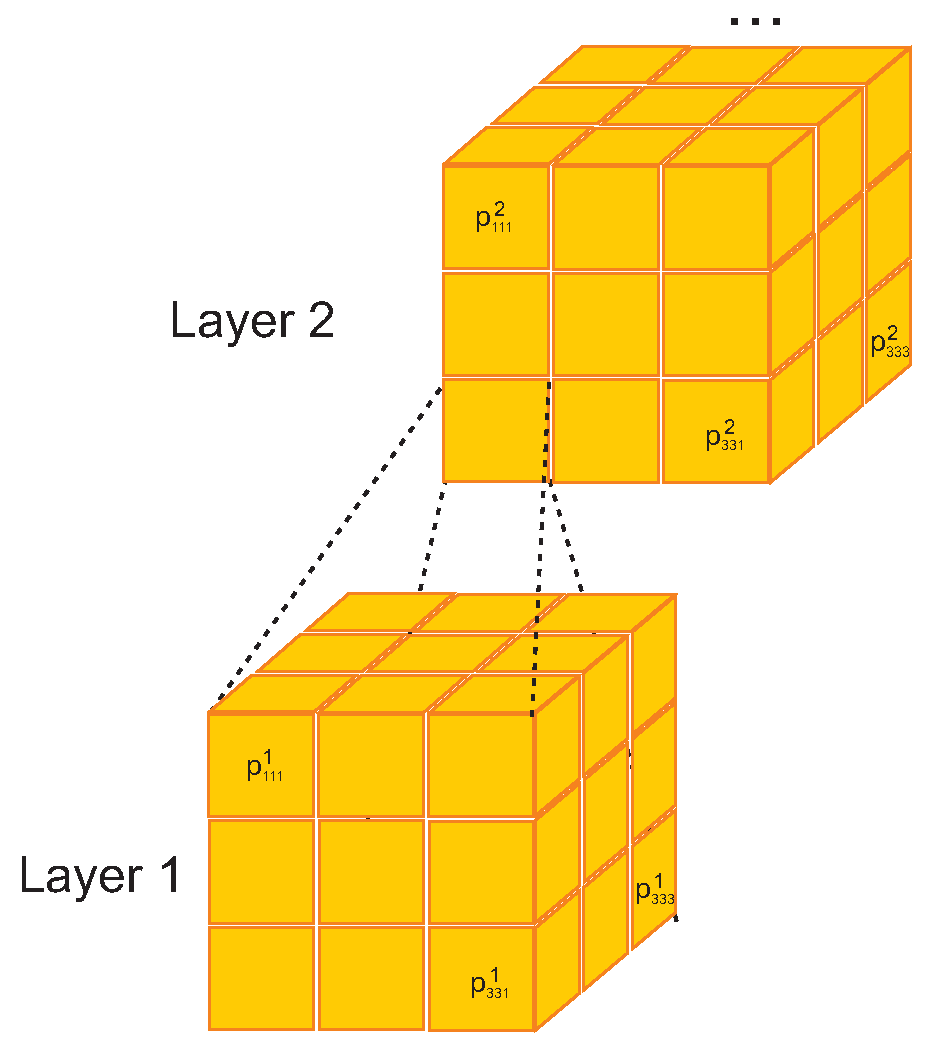
\includegraphics[width=0.75\columnwidth]{../images/wordInd.eps}
% \caption{Representation of words in the view-invariant layers}
%  \label{wordInv}
% \end{figure}

The general learning principle is the same for view-variant and view-invariant layers (Fig.~\ref{hopProc}). For view-invariant layers the receptive field is a cube. The relation between words from $i$ and $i+1$ layers is presented in Fig.~\ref{word}. A word in the $i+1^{th}$ layer consists of 27 words (parts) from the $i^{th}$ layer. The receptive fields for the volumetric layers grow in three dimensions.

To create the first layer of the volumetric vocabulary we transform each part from the view-dependent layer into 3D using the known position of the camera for each viewpoint. In our current implementation we start to build volumetric layers from parts of the second view-dependent layer. Then, we hierarchically convert each part into a point cloud. We store the points for each object in separate octrees. To reduce the number of points and to combine information about surfaces observed from many viewpoints we run voxel grid filtering~\cite{Aldoma2012}. In contrast to~\cite{Aldoma2012} we preserve normal vectors for each voxel. During computation of the mean point for each voxel the points are clustered according to the normal vector. The maximal distance (angle) between normal vectors inside single cluster is set to 45$^\circ$. For each obtained cluster the mean position and normal vector is computed. This approach allows us to preserve the inner and outer surfaces of the objects.

\begin{figure}[t]
 \centering
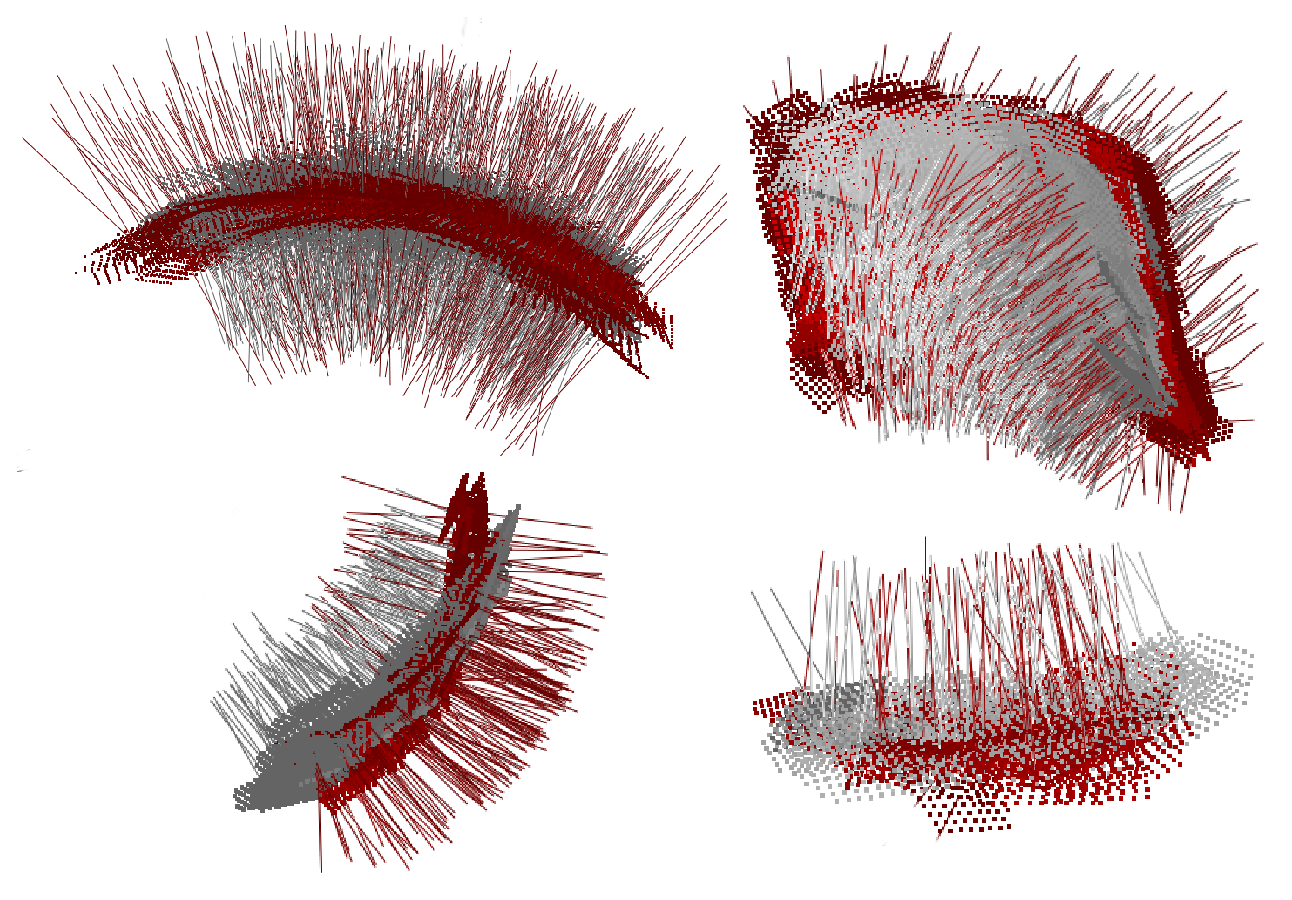
\includegraphics[width=0.95\columnwidth]{../images/viParts.eps}
\caption{Alignment of parts from the fourth layer. Gray -- part A ($p_A$), red -- part B ($p_B$)}
 \label{viParts}
\end{figure}

To compute the similarity between pairs of view-invariant parts we find the SE(3) transformation $T$ which aligns two parts. To find the optimal transformation $T$ we minimize the error:

\begin{equation}
\label{optVol}
 \arg\min_{\bf T} (n_A-n_B)^2 \sum_i ||{\bf N}_B^i \cdot ({\bf T}\cdot {\bf p}_A^{\rm i}-{\bf p}_B^{\rm i})||^2,
\end{equation}

where ${\bf p}_A^{\rm i}$ and ${\bf p}_B^{\rm i}$ are corresponding points from part A and part B, $n_A$ and $n_B$ are the number of points in the respective parts, ${\bf N}_B^i$ is the surface normal at ${\bf p}_B^{\rm i}$. The element $(n_A-n_B)^2$ in (\ref{optVol}) is added to prevent matching parts with significantly different size. To find the correspondences between points and to compute the optimal transformation $T$ we use a point-to-plane variant of Iterative Closest Point~\cite{Segal2009}. To prevent sub-optimal solutions we run ICP multiple times. Each optimization starts from a randomly initialized initial guess. Because the positions of points are defined in the centre of the part we only randomly initialize the orientations of the parts. 

The example alignment of parts from the fourth layer is presented in Fig.~\ref{viParts}. In contrast to parts from view-dependent layers, which represent single surfaces, the parts from volumetric layers can contain multiple surfaces. View invariant parts from volumetric layers represent, for example, both the inner and outer surfaces of the objects (cf. Fig.~\ref{parts3rdLayer} and Fig.~\ref{parts2ndLayer}).

The procedure for part selection is the same as for view-dependent layer. When the next layer vocabulary is selected, the receptive fields are increased and the part extraction procedure is repeated (Fig.~\ref{hopProc}). To minimize the influence of the object pose in relation to the global coordinate system the view-invariant receptive fields are also shifted by 33\%. This strategy also provides redundant information about parts covered by receptive fields. Thus, the identification of parts for problems such as grasping is more robust.

\section{Results}

\begin{figure}[t]
 \centering
\includegraphics[width=0.95\columnwidth]{../images/shareability.eps}
\put(-230,205){a} \put(-230,85){b}
\put(-162,236){c}\put(-82,237){d} 
\caption{Shareablity of parts from view-dependent layers between two categories of objects (bowl (a) and mug (b)) for: second (c) and third (d) layer parts of the hierarchy}
 \label{shareability}
\end{figure}

The learning of the hierarchy allows us to find parts which explain the input data. The most important property of the hierarchy is shareability. The parts are shared between object categories. Thus inference and activities such as grasping can be also transfered from the training object to another object. The shareability of parts from view-dependent layers is presented in Fig.~\ref{shareability}. This shareability property is presented for two types of objects: mug and bowl. In Fig.~\ref{shareability}c parts from second layers are presented. The parts which represent concave surfaces (green) can be found on the surface of the mug which is visible from two different viewpoints, as well as on the inner surface of the bowl. Convex parts (pink) are mainly visible on the outer surface of the mug. Some realizations of convex parts can also be found on the bowl's surface, but they only represent the local shape of the surface.

The shareability of parts is also visible on the 3rd layer of the hierarchy (Fig.~\ref{shareability}c). Because the size of the receptive field is bigger than the size of the first layer's receptive field also the difference between qualitative geometric properties of surfaces (convexity vs. concavity) are better visible. The same part realizations can be found on the surface of the mug and on the surface of the bowl (concave parts are represented by the colour purple).

\begin{figure}[t]
 \centering
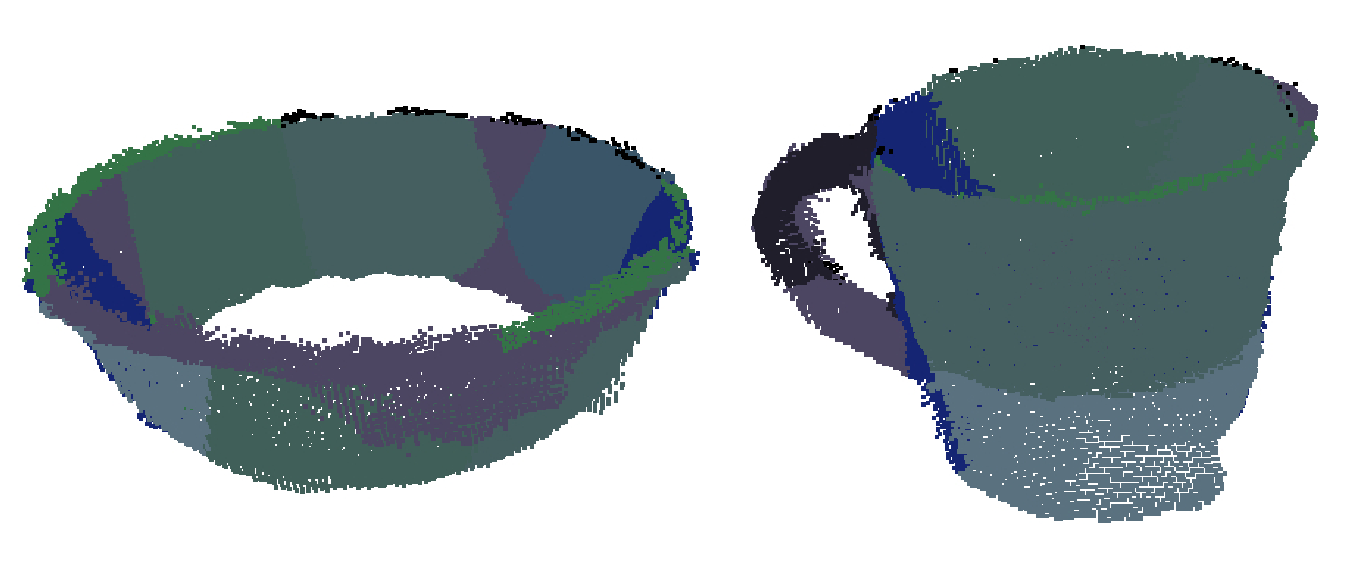
\includegraphics[width=0.95\columnwidth]{../images/shareability4thLayer.eps}
\put(-227,80){a} \put(-100,80){b}
\caption{Shareablity of 4th layer parts between objects.}
 \label{shareability4thLayer}
\end{figure}

The shareability of parts can be also observed in volumetric layers of the hierarchy (Fig.~\ref{shareability4thLayer}). Some parts represent edges (green and purple), and other, bigger parts correspond to the inner and outer surfaces of the object are shared between the mug and the bowl. Note that some parts which are related to the edges can be also found on the objects' surfaces (purple parts in Fig.~\ref{shareability4thLayer}a). This is the result of the receptive fields forming a regular grid. The positions of the receptive fields in 3D strongly influence how the object is divided into parts. To mitigate this problem we implemented overlapping receptive fields. The information about spurious edges can be also ignored because the location of the edge is not supported by parts from lower layers of the hierarchy.

\begin{figure}[t]
 \centering
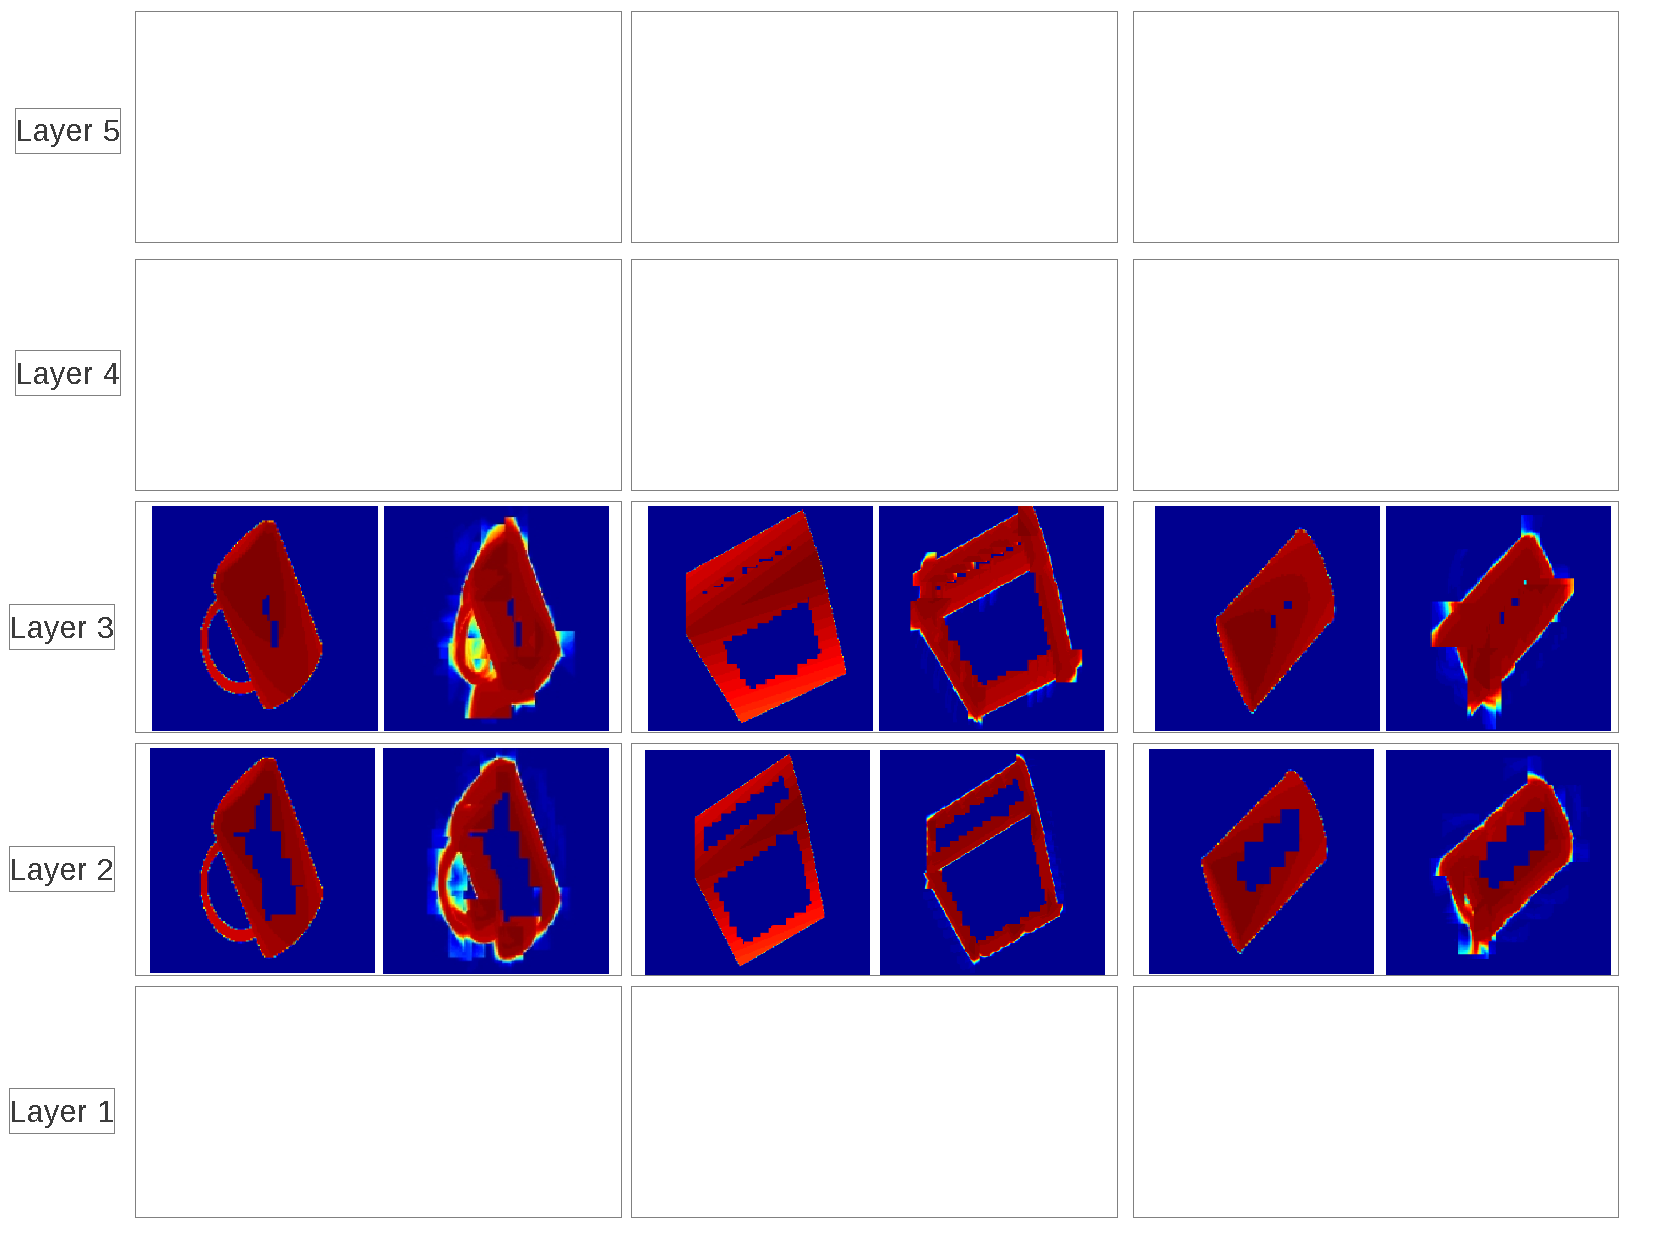
\includegraphics[width=1.0\columnwidth]{../images/inference.eps}
\put(-240,260){a} \put(-180,260){b} \put(-120,260){c} \put(-55,260){d}
\caption{Inference results for five new objects (a): parts obtained on the second (b), third (c) and fourth (d) layers. The shareability of parts obtained during training the hierarchy is presented in Fig.~\ref{shareability} and Fig.~\ref{shareability4thLayer}.}
 \label{inference}
\end{figure}

\addtolength{\textheight}{-12cm}  

% \section*{APPENDIX}

% Appendixes should appear before the acknowledgment.

% \section*{ACKNOWLEDGMENT}
% acknowledgment

\begin{thebibliography}{99}
\bibitem{Aldoma2012}
A. Aldoma, Z.C. Marton, F. Tombari, W. Wohlkinger, C. Potthast, B. Zeisl, R.B. Rusu, S. Gedikli, M. Vincze, Point cloud library: Three-Dimensional Object Recognition and 6 DoF Pose Estimation. IEEE Robotics \& Automation Magazine, pp.~80-91, 2012
\bibitem{Fiedler2014}
  S. Fidler, M. Boben, A. Leonardis, Learning a Hierarchical Compositional Shape Vocabulary for Multi-class Object Representation, Computer Vision and Pattern Recognition, 2014 (under review)
\bibitem{Riesenhuber1999}
M. Riesenhuber, T. Poggio,Hierarchical models of object recogni-tion in cortex. Nature Neuroscience, Vol.~2, pp.~1019--1025, 1999
\bibitem{Serre2007}
T. Serre, G. Kreiman, M. Kouh, C. Cadieu, U. Knoblich, T. Poggio, A quantitative theory of immediate visual recognition. Progress in
Brain Research, Vol.~165, pp.~33--56, 2007
\bibitem{Spehr2015}
J. Spehr, On Hierarchical Models for Visual Recognition and Learning of Objects, Scenes, and Activities, Studies in Systems, Decision and Control, Springer, 2015
\bibitem{Umeyama1991}
 S. Umeyama,
 ``Least-squares estimation of transformation parameters between two point patterns'',
 IEEE Trans. on Pattern Analysis \& Machine Intelligence, 13(4), 1991, 376--380.
 \bibitem{Manning2008}
 C. D. Manning, P. Raghavan, H. Sch\"{u}tze, Introduction to Information Retrieval, Cambridge University Press. 2008
 \bibitem{Segal2009}
 A. V. Segal, D. Haehnel, and S. Thrun, Generalized-ICP, Robotics: Science and Systems, 2009
\end{thebibliography}

\end{document}